%---------------------------------------------------------------------------------------
% An Explosive Transition
%---------------------------------------------------------------------------------------
\section{An "Explosive" Transition}
In this paper we are going to take a deeper look into a specific type of percolation called explosive percolation, where the underlying concept is that the onset of percolation is delayed until a certain point where it then occurs at an accelerated rate.
This occurs when the underlying evolution process works in such a way that the largest cluster size $|C|$ is controlled.
We can think of a graph where multiple clusters might evolve separately without merging.
Collectively they take up a large portion of the graph but there isn't a percolating cluster yet due to the lack of connections between the them.
If at some point these clusters do begin to connect then the graph transitions to the percolating state.
For certain evolution processes it has been heavily debated whether or not the phase transition is continuous or not, so the aim of the next section is to summarize what we know to this point regarding the nature of the transition for said processes.



%---------------------------------------------------------------------------------------
% A Selective Process
%---------------------------------------------------------------------------------------
\subsection{A Selective Process}
This all started in the year 2000 when Dimitris Achlioptas raised an interesting question about how a graph of $N$ nodes would evolve under certain conditions \cite{BF}.
First we suppose that at each step $t$ in the evolution process two edges $e_t$ and $e_t'$ are evaluated, but only one of them is selected to be added to the graph.
Which of the proposed edges is selected is based only on the information contained in $e_1, e_1', ... e_{t-1}, e_{t-1}'$.
Does there exist an algorithm for adding edges to the graph such that with high probability a giant component does not appear until $t/N > 0.5$?
This process of evaluating $m \ge 2$ edges at each step is now referred to as an $q$-edge Achlioptas process.
In the next few sections we will see how a small change to the way edges are added can have a big impact on the evolution of the system.



%---------------------------------------------------------------------------------------
% The First Look
%---------------------------------------------------------------------------------------
\subsection{The First Look}
In 2001 Tom Bohman and Alan Frieze were the first to design and analyze an Achlioptas process in their paper "Avoiding a Giant Component" \cite{BF}, where they set out to answer Achlioptas' question.
This paper laid out the framework for the Bohman-Frieze (BF) model of graph evolution and showed that there does exist a process in which the appearance of a giant cluster is delayed; so the answer to Achlioptas' question is yes!
This can be seen in Fig. \ref{fig:ER_BF_transition} where the order parameter for the BF model remains smaller than for the ER model, but a little after $r = 0.5$ it begins to rise at a faster rate than in the ER model, eventually overtaking the ER model.

\begin{figure}[H]
	\centering
	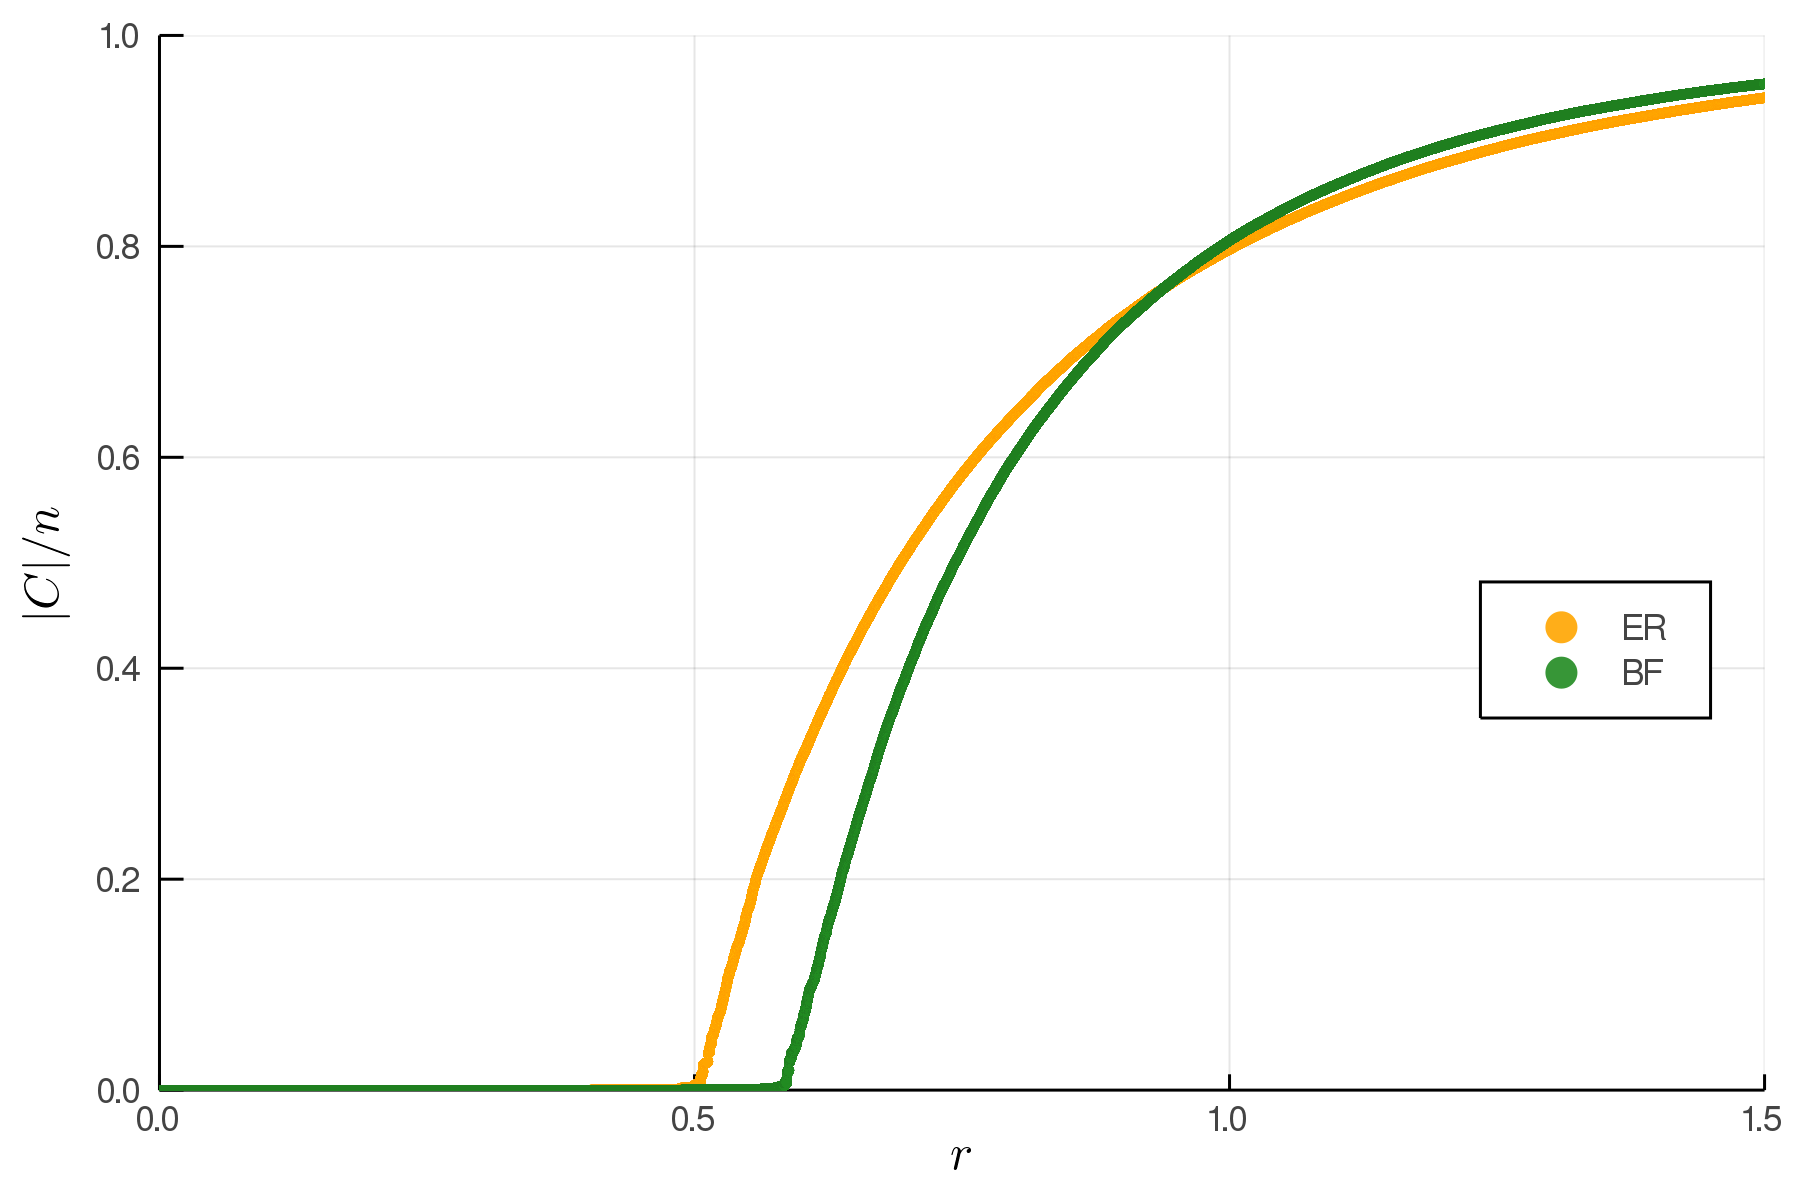
\includegraphics[width=350pt]{images/Network_ER_BF_1e6_order_param.png}
	\caption{Bohman-Frieze Model Order Parameter, $N = 10^6$}
	\label{fig:ER_BF_transition}
\end{figure}

The algorithm they came up with randomly/uniformly samples and evaluates two edges $e_t$ and $e_t'$ at each step $t$, adding $e_t$ if it connects two isolated nodes and discarding $e_t'$, otherwise adding $e_t'$ and discarding $e_t$.
This is known as a bounded-size rule, which has since been generalized to a $K$ bounded-size rule where $e_t$ is added if it connects clusters of size smaller than $K$, otherwise $e_t'$ is added.
What this process does is equally discriminate against clusters of size greater than or equal to $K$.
It has been hypothesized that all bounded-size rules exhibit continuous phase transitions \cite{Spencer_Wormald}.

A form of the algorithm can be written in pseudocode as follows:
\begin{itemize}
	\item Let $T$ be the total number of edges to add to the graph.
	\item Let $A_t = \{e_1, e_2, ..., e_t\}$ be the set of accepted edges at step $t$.
	\item Let $e_t^1$ and $e_t^2$ be the two nodes which edge $e_t$ would connect.
	\item Let $C(e_t^i)$ be the cluster which $e_t^i$ belongs to.
\end{itemize}

\begin{algorithm}
	\caption{Bohman-Frieze}\label{Bohman-Frieze}
	\begin{algorithmic}[1]
		\Procedure{BF}{$T, K=2$}
		\State $A \gets \emptyset$
		\State $t \gets 1$
		\While{$t \le T$}
			\If{$|C(e_t^1)| < K$ and $|C(e_t^2)| < K$}
				\State $A \gets A \cup \{e_t\}$
			\Else
				\State $A \gets A \cup \{e_t'\}$
			\EndIf
			\State $t \gets t+1$
		\EndWhile
	\EndProcedure
	\end{algorithmic}
\end{algorithm}

A few years after their original paper, Bohman and Frieze published another paper with Nicholas Wormald titled "Avoidance of a giant component in half the edge set of a random graph" \cite{BFW}.
In this paper they designed a new algorithm (BFW) for adding edges to a graph that runs in phases beginning at $k = 2$.
Starting with $N$ isolated nodes, edges are randomly/uniformly sampled and evaluated one at a time.
If the edge being evaluated would create a cluster of size less than or equal to $k$ then the edge is accepted, otherwise the edge is rejected.
If edge is rejected and the ratio of accepted edges is less than the function $g(k) = 1/2 + \sqrt{1/(2k)}$, then the algorithm moves to the next phase.

A form of the algorithm can be written in pseudocode as follows:
\begin{itemize}
	\item Let $T$ be the total number of edges to add to the graph.
	\item Let $A_i = \{e_1, e_2, ..., e_i\}$ be the set of accepted edges at step $i$.
	\item Let $C(A)$ be the largest cluster in $A$.
\end{itemize}

\begin{algorithm}
	\caption{Bohman-Frieze-Wormald}\label{Bohman-Frieze-Wormald}
	\begin{algorithmic}[1]
		\Procedure{BFW}{$T$}
		\State $A \gets \emptyset$
		\State $k \gets 2$
		\State $t \gets 1$
		\State $i \gets 1$

		\While{$t \le T$}
			\If{$|C(A \cup \{e_i\})| \le k$}
				\State $A \gets A \cup \{e_i\}$
				\State $t \gets t+1$
				\State $i \gets i+1$
			\ElsIf{$|A|/i < g(k)$}
				\State $k \gets k+1$
			\Else
				\State $i \gets i+1$
			\EndIf
		\EndWhile
	\EndProcedure
	\end{algorithmic}
\end{algorithm}



%---------------------------------------------------------------------------------------
% A Discontinuous Transition
%---------------------------------------------------------------------------------------
\subsection{A Discontinuous Transition?}
The first mention of explosive percolation appeared in 2009 in the paper "Explosive Percolation in Random Networks" \cite{Achlioptas_1} by Dimitris Achlioptas, Raissa M. D’Souza, and Joel Spencer, which will henceforth be referred to as Achlioptas et al.
In this paper they laid out a method of choosing edges called the product rule (PR).
At each step $t$ in the evolution process two edges are selected randomly/uniformly and evaluated based on the product of the cluster sizes that the edges would connect.
More specifically, if edge $e_t$ connects clusters $C(e_t^1)$ and $C(e_t^2)$ and edge $e_t'$ connects clusters $C(e_t'^1)$ and $C(e_t'^2)$, then $e_t$ is accepted if $|C(e_t^1)| \cdot |C(e_t^2)| < |C(e_t'^1)| \cdot |C(e_t'^2)|$, otherwise $e_t'$ is accepted.

A form of the algorithm can be written in pseudocode as follows:
\begin{itemize}
	\item Let $T$ be the total number of edges to add to the graph.
	\item Let $A_t = \{e_1, e_2, ..., e_t\}$ be the set of accepted edges at step $t$.
	\item Let $e_t^1$ and $e_t^2$ be the two nodes which edge $e_t$ would connect.
	\item Let $C(e_t^i)$ be the cluster which $e_t^i$ belongs to.
\end{itemize}

\begin{algorithm}
	\caption{Product Rule}\label{Product-Rule}
	\begin{algorithmic}[1]
		\Procedure{PR}{$T$}
		\State $A \gets \emptyset$
		\State $t \gets 1$

		\While{$t \le T$}
			\If{$|C(e_t^1)| \cdot |C(e_t^2)| < |C(e_t'^1)| \cdot |C(e_t'^2)|$}
				\State $A \gets A \cup \{e_t\}$
				\State $t \gets t+1$
			\Else
				\State $A \gets A \cup \{e_t'\}$
				\State $t \gets t+1$
			\EndIf
		\EndWhile
	\EndProcedure
	\end{algorithmic}
\end{algorithm}

This is illustrated in Fig. \ref{fig:edge_selection} where the first proposed edge $e_t$ would connect the blue cluster of size 5 to the red cluster of size 3 and the second proposed edge $e_t'$ would connect the orange cluster of size 2 to the green cluster of size 4.
The product corresponding to $e_t$ is $5 \cdot 3 = 15$ whereas the product corresponding to $e_t$ is $2 \cdot 4 = 8$, so $e_t$ is rejected and $e_t'$ accepted.
If we were looking at Fig. \ref{fig:edge_selection} from within the framework of the BF model with $K = 1$, then $e_t$ would be rejected and $e_t$ accepted even though both the orange and green clusters are of size greater than $K$.

\begin{figure}[H]
	\centering
	\includegraphics[width=200pt, clip]{images/edge_selection.png}
	\caption{Edge Selection}
	\label{fig:edge_selection}
\end{figure}

Fig. \ref{fig:ER_BF_PR_transition} shows the order parameters for the ER, BF, and PR models, making it clear just how drastically different the PR model transition is than in the ER/BF models.
As can be seen the order parameter remains near zero for much longer until the critical point $r_c \approx 0.888...$, which is much later than the critical point in the ER model of $r_c = 0.5$.
Not long after the critical point is reached the order parameter appears to jump up discontinuously, which was a surprising find.

\begin{figure}[H]
	\centering
	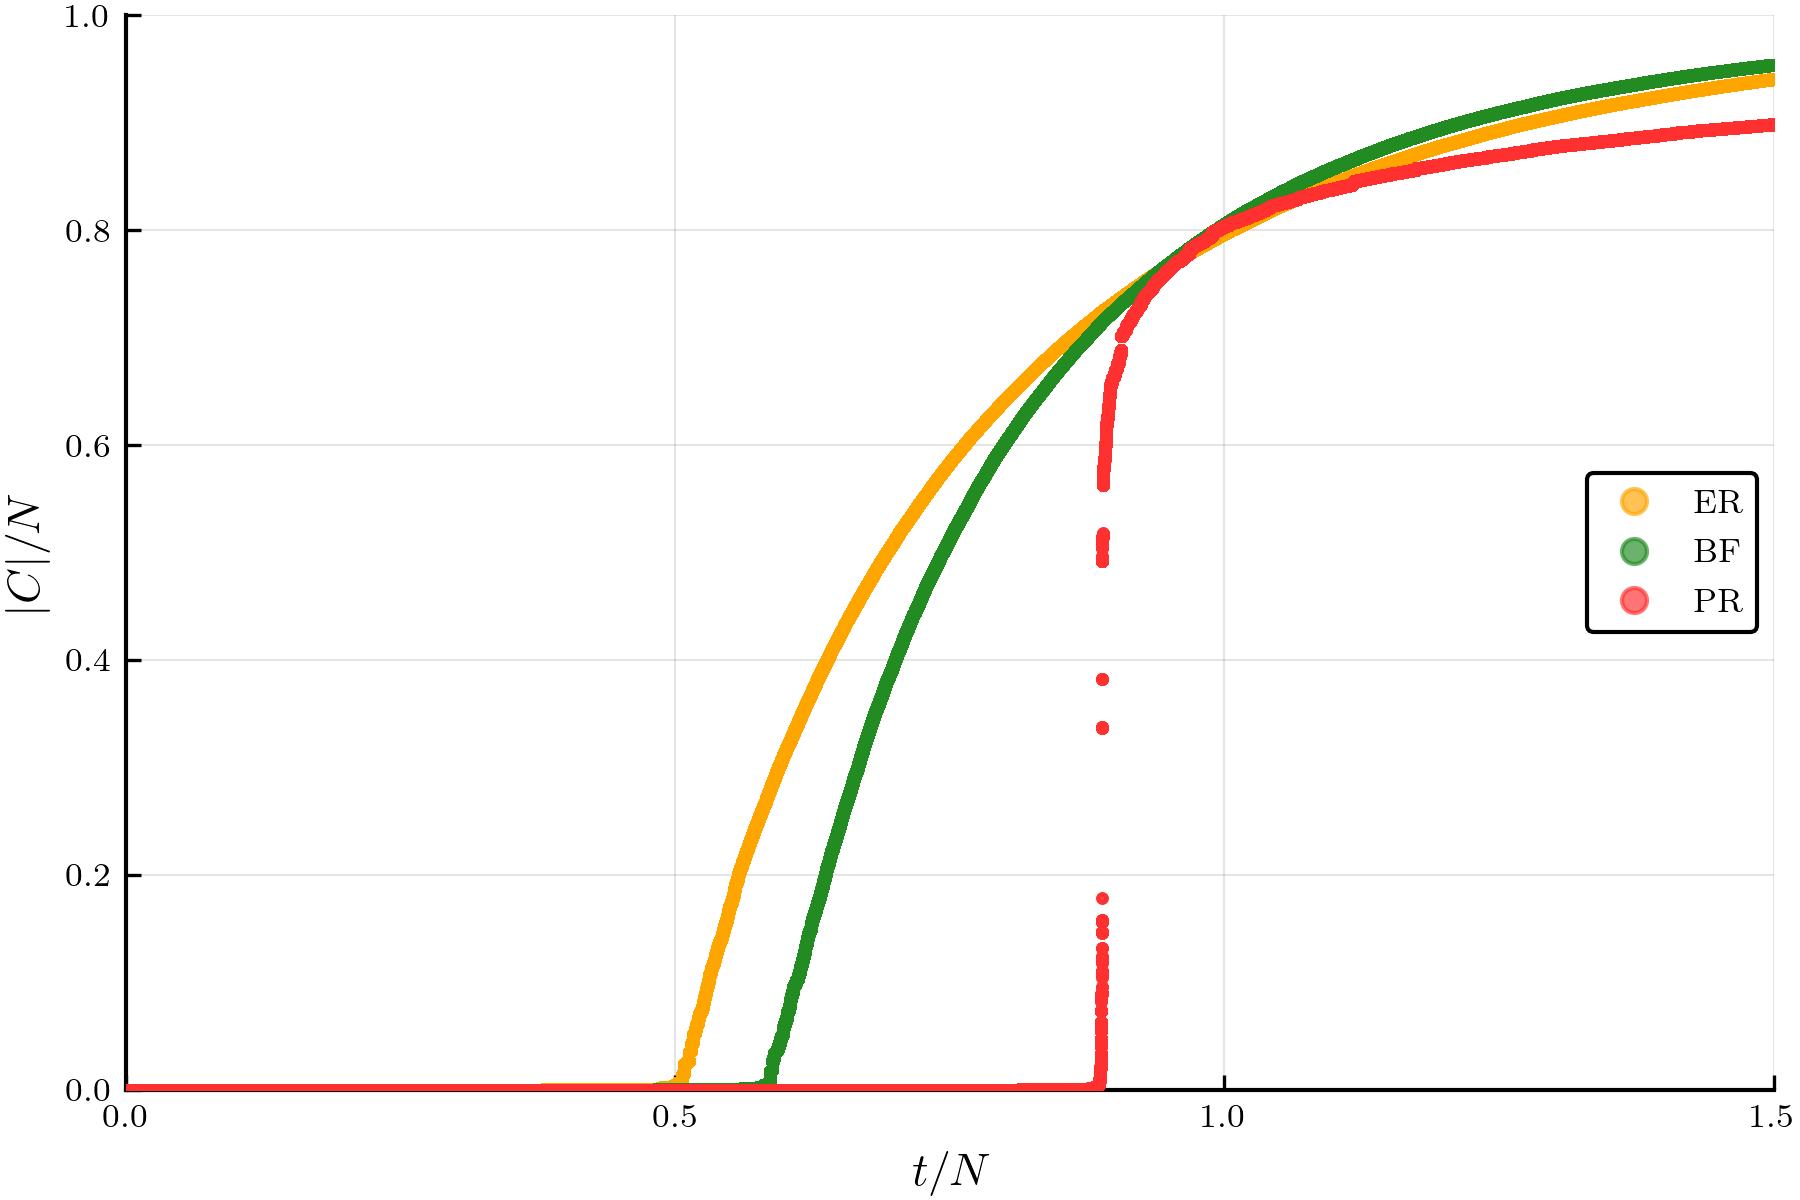
\includegraphics[width=350pt]{images/Network_ER_BF_PR_1e6_order_param.png}
	\caption{Product Rule Model Order Parameter, $N = 10^6$}
	\label{fig:ER_BF_PR_transition}
\end{figure}

In their paper they analyzed the scaling behavior of their model, defining the quantity $\Delta := t_1 - t_0$, where $t_0$ is the last step where $C < N^{1/2}$ and $t_1$ is the first step where $C > 0.5N$.
$\Delta$ is linear in $N$ for continuous transitions (i.e. an extensive quantity), however, their analysis indicated otherwise that $\Delta < 2N^{2/3}$ and $\Delta / N^{2/3} \rightarrow 1$ in their simulations for sizes up to $6.4 \cdot 10^7$.
To arrive at these results they took an ensemble average of 50 different independent and identically distributed observations and fit a curve to determine the relation between $\Delta$ and $N$.
Their findings are illustrated in Fig. \ref{fig:achlioptas_plots}.

\begin{figure}[H]
	\centering
	\includegraphics[width=400pt]{images/achlioptas_plots.png}
	\caption{Achlioptas et al. Simulation Results, Source: \cite{Achlioptas_1}}
	\label{fig:achlioptas_plots}
\end{figure}

They ended their paper by saying: "We have demonstrated that small changes in edge formation have the ability to fundamentally alter the nature of percolation transitions. Our findings call for the comprehensive study of this phenomenon, and of its potential use in bringing phase transitions under control."
Indeed their message seemed to resonate, leading to a wave of papers from around the world exploring the subject \cite{Ziff_1, Cho_1, Radicchi_1, Friedman_1, Ziff_2, Radicchi_2, D_Souza_1, da_Costa_1, Rozenfeld_1, Araujo_1, Moreira_1, Cho_2, Cho_3, Nagler_1, Manna_1, Grassberger_1, Lee_1, Riordan_1, Hooyberghs_1, Nagler_2, Chen_1, Panagiotou_1, Pan_1, Cho_4, Gomez_1, Tian_1, Riordan_2, Riordan_3, Boettcher_1, Chen_2, Angst_1, Bizhani_1, Cho_5, Schroeder_1, Chen_3, Chen_4, Squires_1, Do_1, Chen_5, Bastas_1, Cho_6, da_Costa_2, Riordan_4, Guan_1, da_Costa_5, da_Costa_3, da_Costa_4, D_Souza_2, Hayasaka_1, Clusella_1, Boccaletti_1, Gedik_1, Rahman_1, Waagen_1, Zhu_1, Sabbir_1, Trevelyan_1, Sabbir_1}.



\subsubsection{No, It's Actually Continuous!}
In 2010 Rui da Costa, Sergey Dorogovtsev, Alexander Goltsev, and Jose Fernando Mendes published \cite{da_Costa_1} wherein they dispute that the explosive percolation transition is actually continuous.
They used an edge selection rule which at each step chooses two sets of $q$ nodes, determines for each set the node belonging to the smallest cluster, then activates the edge between those to thus favoring the merging of smaller clusters and minimizing the largest cluster in the process.
They were able to show power law behavior of the largest cluster size for $m = 2$:

\begin{equation}
	|C| \propto \delta^\beta
\end{equation}
where $\delta = |r - r_c|$, with $t_c = 0.923207508(2)$ and $\beta = 0.0555(1)$ which is close to $1/18 = 0.055\overline{5}$.

They then show that if the cluster size distribution is power law distributed at the critical point then the transition must be continuous.
Their paper concludes by saying reason it is difficult to distinguish this transition from a discontinuous one is due to the small value of $\beta$, and that due to the irreversibility of the process that it is an attractive subject to further develop.



\subsubsection{Well, Maybe Not...}
In their paper "Explosive Percolation with Multiple Giant Components" \cite{Chen_1}, Wei Chen and Raissa M. D’Souza took a modified version of the BFW model mentioned above.
They took the parameter $\alpha$ which is the asymptotic fraction of accepted edges and demonstrated that changing $\alpha$ determines the number of stable giant clusters.
The smaller the value of $\alpha$ the longer the transition will be delayed and the more explosive it will be.
This is shown in Fig. \ref{fig:bfw_alpha_comparison}

\begin{figure}[H]
	\centering
	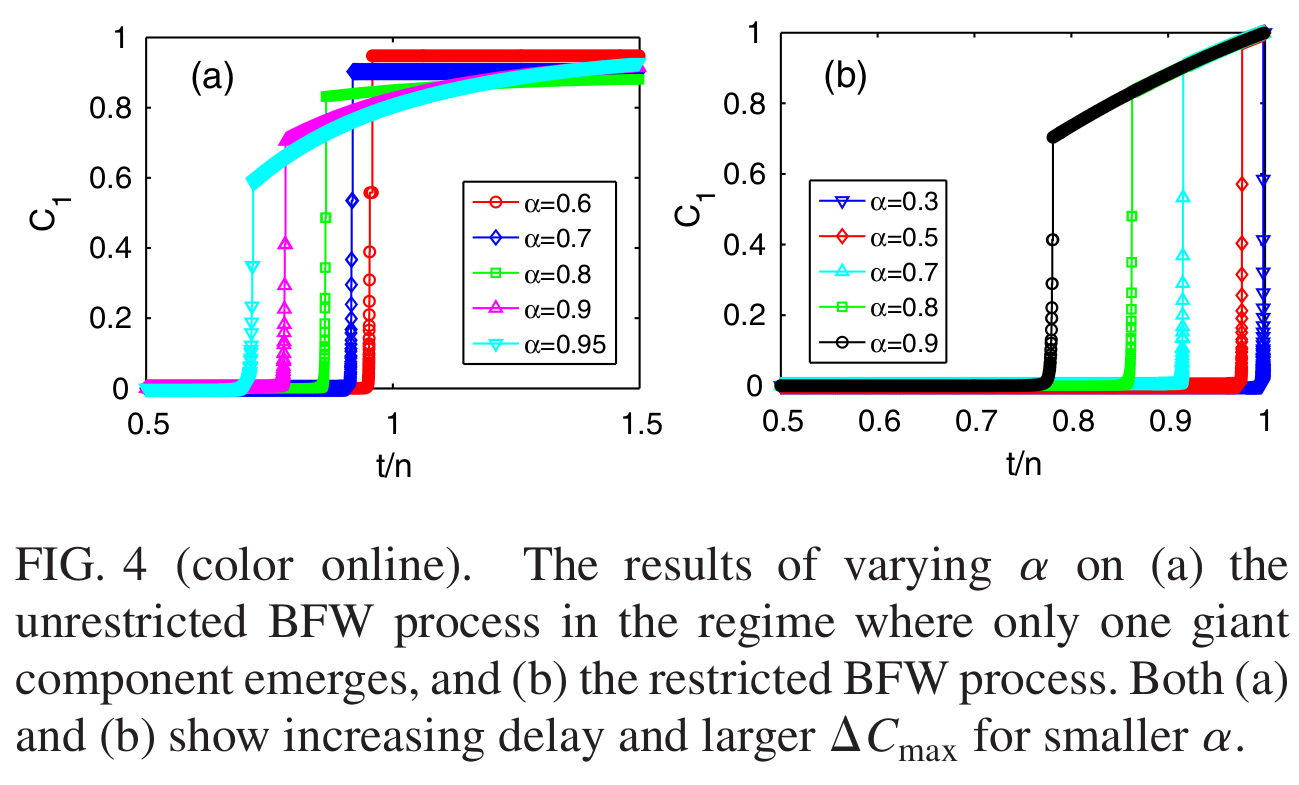
\includegraphics[width=350pt]{images/bfw_alpha_comparison.png}
	\caption{Phase Transition Dependence on $\alpha$, Source: \cite{Chen_1}}
	\label{fig:bfw_alpha_comparison}
\end{figure}

Their analysis shows that it is possible to have multiple stable giant components emerge at the same critical point.
Furthermore they finish their paper by stating that the BFW model is strongly discontinuous.



\subsubsection{Continuity With Unusual Finite-Size Scaling Behavior}
In 2011 Grassberger et al. published "Explosive Percolation is Continuous, but with Unusual Finite Size Behavior" \cite{Grassberger_1} in which they studied the phase transitions of four different Achlioptas processes.
They specifically look at the distribution $P_{r, N}(m)$ of the order parameter $m = |C| / N$, and at criticality it scales as:

\begin{equation}
	P_{r=r_c, N}(m) \sim N^\eta f(m N^\eta)
\end{equation}
In the Ising model (continuous transition) the function $f(z)$ has two peaks and as $N \rightarrow \infty$ the peaks move closer together to form a single peak, whereas in a first order transition $f(z)$ is double peaked and the peaks move further apart as $N \rightarrow \infty$.
The finite size scaling of $\langle m \rangle$ is given by:

\begin{equation}
	\langle m \rangle \sim (r - r_c)^\beta g((r - r_c) N^\Theta)
\end{equation}
$g(z)$ is analytic for all $z \in \mathbb{R}$.

\begin{figure}[H]
	\centering
	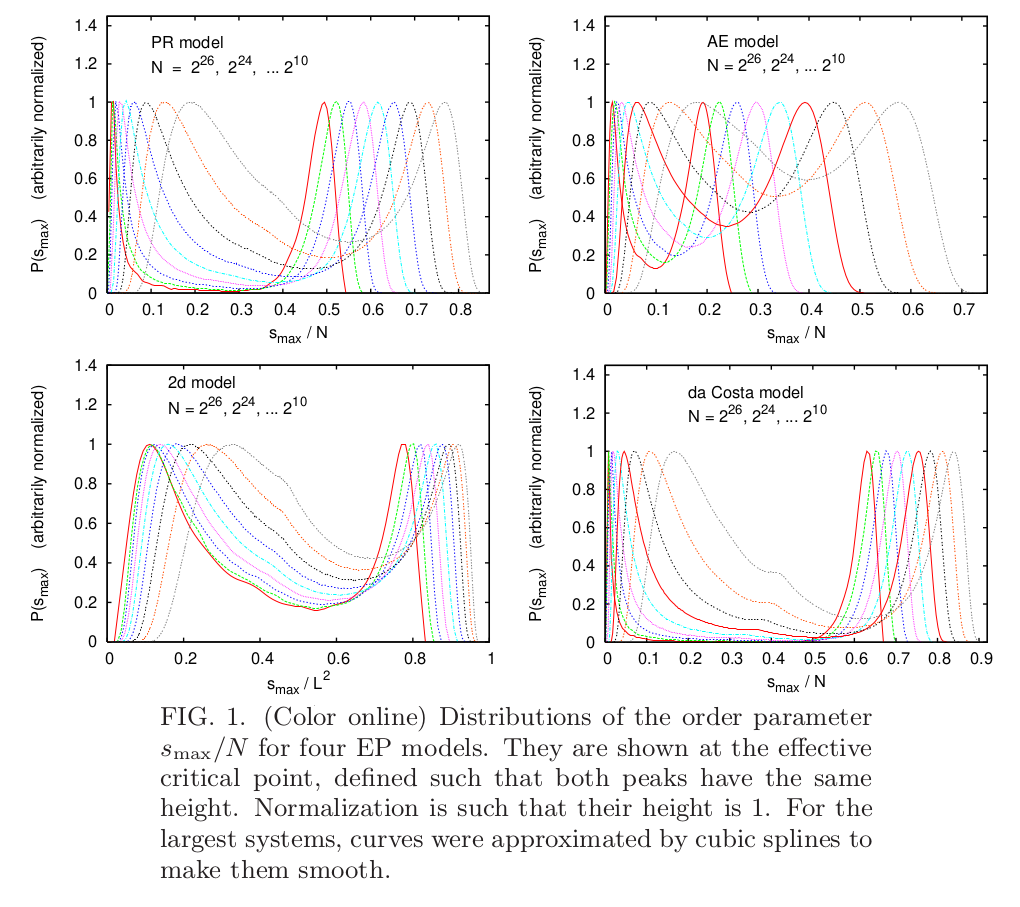
\includegraphics[width=350pt]{images/grassberger_scaling.png}
	\caption{Scaling of $P_{r=r_c, N}(m)$, Source: \cite{Grassberger_1}}
	\label{fig:grassberger_scaling}
\end{figure}

Their results, shown in Fig. \ref{fig:grassberger_scaling} showed that $P_{r=r_c, N}(m)$ was indeed double peaked, however, they say that this does not prove it is continuous, rather it reflects how abruptly the system transitions.
They then go on to show (through the use of FSS of $\langle m \rangle$) that the transitions of the studied four models are indeed continuous, yet are each in a different universality class and all exhibit unusual finite size scaling behavior.



\subsubsection{Large Scale Simulations Show It's Continuous}
The 2011 paper "Continuity of the Explosive Percolation Transition" \cite{Lee_1} by Hyun Keun Lee, Beom Jun Kim, and Hyunggyu Park analyzed the finite-size scaling of the product rule in depth, using data from simulations of system sizes up to $2^{37} \approx 1.4 \cdot 10^{11}$.
They use a fairly straightforward method for determining the continuity of the transition:

\begin{enumerate}
	\item Set $t_0(N) < t_c$ and $t_1(N) > t_c$ with the expectation that as $N \rightarrow \infty$, $t_0 \rightarrow t_c$ and $t_1 \rightarrow t_c$.
	\item Find an upper bound for the change in the largest cluster size $\Delta |C|$.
	\item Show that $\Delta |C|$ scales sublinearly with $N$.
\end{enumerate}

Near the end they arrive at:

\begin{equation}
	\Delta m = \frac{\Delta |C|}{N} \lesssim N^{-0.022}
\end{equation}
Which means that as $N \rightarrow \infty$, $\Delta m \rightarrow 0$ and they conclude that the transition is indeed continuous.



\subsubsection{Proof of Continuity Emerges}
Oliver Riordan and Lutz Warnke published "Achlioptas Process Phase Transitions Are
Continuous" \cite{Riordan_1} in 2012, wherein they lay out several theorems and proofs to show that all Achlioptas processes result in a continuous phase transition.
Due to the long and detailed nature of the proofs I will refer the reader to their work for further information.



\subsubsection{"Solution of the explosive percolation quest"}
In 2014 and 2015 Rui da Costa, Sergey Dorogovtsev, Alexander Goltsev, and Jose Fernando Mendes published three more papers \cite{da_Costa_5, da_Costa_2, da_Costa_3} where they performed a significant amount of research on the explosive percolation transition of the $q$-edge model laid out in their previous paper (see above \textbf{No, It's Actually Continuous!}).

In "Critical exponents of the explosive percolation transition" \cite{da_Costa_5} they study extensively the critical exponents and how they scale as $q$ changes, wherein they observe that as $q$ increases $\beta$ quickly declines, with $\beta(q = 4) \approx \beta(q = 2) / 20$.
They talk about how models that only use local information, i.e. they do not require knowledge of all of the clusters within the graph but only those corresponding to the candidate edges, lead to a continuous transition, but models that take global information into account might lead to discontinuities.

In "Solution of the explosive percolation quest: Scaling functions and critical exponents" \cite{da_Costa_2}
and "Solution of the explosive percolation quest. II. Infinite-order transition produced by the initial distributions of clusters" \cite{da_Costa_3} they develop a thorough theory of finite-size scaling that explains the continuity of the transition.
Their theory is quite extensive, therefore, I must refer the reader to their work for more information.



\subsubsection{A Look At the Developments}
After seeing a number of papers stating that the transition is actually continuous, it looked like the debate had been settled.
$q$-edge Achlioptas processes are always continuous if they only take local information into account, but there exist some processes that take global information into account that lead to a discontinuous transition.
A lot of different rules for selecting, evaluating, and adding edges were created and in the 2015 paper "Explosive Percolation: Novel critical and supercritical phenomena" \cite{D_Souza_2} by Raissa M. D’Souza and Jan Nagler summarized a lot of the developments and findings in the field up to that point.
They discussed similarities and differences between some of the well known explosive percolation models and tied it all together nicely some real world applications and future directions for the field.
Overall it is an excellent paper to read to get acquainted with how the field developed from 2009 to 2015.
